\chapter{Решение в двумерном случае}
\section{Постановка задачи}
 

 Рассмотрим наклонное падение монохроматической плоской TM-волны на две полубесконечные металлические пластины (Рис.~\ref{fig:geom}). 
 Тогда y-компонента магнитного поля будет подчиняться однородному волновому уравнению 
 \begin{equation}
   \frac{\partial^2 H}{\partial x^2} +   \frac{\partial^2 H}{\partial y^2} = \frac{\epsilon}{c^2}\frac{\partial^2 H}{\partial t^2}.
 \end{equation}
 Здесь предполагается, что в выбранном диапазоне частот ($\lambda = 1,5$ мкм) золото немагнитное, то есть $\mu = 1$ и $B = H$. Область при $z<0$ 
 и между пластинами является вакуумом, и соответственно для него проницаемость $\eps = 1$, проницаемость металла является
 комплексной величиной $\eps_M = \eps' + i \eps''$, где вещественная часть $\eps'$ отрицательна и $\abs{\eps'} \gg 1$, мнимая же часть 
 отвечает за омические потери, следовательно положительна. 
\begin{figure}
    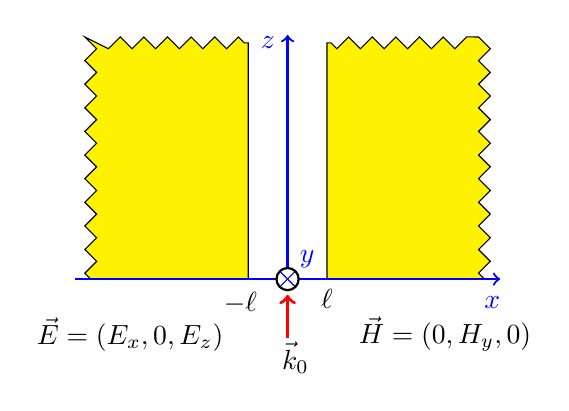
\begin{tikzpicture}[decoration={zigzag,segment length = 3mm, amplitude = 0.75mm}]
        \draw [very thick,red,->] (0,-0.75)--(0,-0.2);
\draw [fill=yellow] (-2.5,0) decorate{--(-2.5,3) -- (-0.5,3)} -- (-0.5,0) -- cycle;
\draw [fill=yellow] (2.5,0) decorate{-- (2.5,3) -- (0.5,3)} -- (0.5,0) -- cycle;
        \draw [blue,thick,->] (-2.7,0)--(2.7,0);
        \draw [black] (0.5,-0.25) node {$\ell$};
        \draw [black] (-0.6,-0.3) node {$-\ell$};
        \draw [blue] (2.6,-0.3) node {$x$};
        \draw [blue,thick,->] (0,0)--(0,3.1);
        \draw [blue] (-0.25,3) node {$z$};
        \draw [thick,fill=white] (0,0) circle (4pt);
        \draw [blue] (-0.09,-0.09)--(0.09,0.09);
        \draw [blue] (0.09,-0.09)--(-0.09,0.09);
        \draw [blue] (0.25,0.25) node {$y$};
        \draw (0.1,-1) node {$\vec{k}_0$};
        \draw (2.0,-0.7) node {$\vec{H} = (0,H_y,0)$};
        \draw (-2.0,-0.7) node {$\vec{E} = (E_x,0,E_z)$};
        \end{tikzpicture}
\caption{Геометрия задачи.}
\label{fig:geom}
\end{figure}

Так как падающее излучение монохроматично, является разумным искать прошедшую в щель и рассеянную на ней волны в том же виде 
$f(t) \sim e^{-i \omega t}$, таким образом задача сводится к решению уравнения Гельмгольца 
 \begin{equation}
   \frac{\partial^2 H}{\partial x^2} +   \frac{\partial^2 H}{\partial y^2} + \eps k_0^2 H = 0,
   \label{eq:Helmholtz}
 \end{equation}
где $k_0 = \omega/c$ --- волновой вектор падающей волны. 

\section{Решение в отдельных подпространствах}
 Для нахождения распределения магнитного поля достаточно найти решение волнового уравнения в обоих полупространствах $z>0$ и $z<0$, а затем их сшить при $z = 0$, используя непрерывность всей полей $\mathbf{E}$ и $\mathbf{H}$. Так как граница $z=0$ неоднородна из-за наличия щели в области
 $\abs{x} < l$, искать решение удобнее всего разделяя переменные как в работах \cite{sturman2010transmission,gorkunov2011transmission}, 
 явным образом выделяя часть, 
 зависящую от $x$. Рассмотрим поля в каждых их подпространств по отдельности.

 \subsection{Поле в области $z < 0$}
В силу линейности уравнения~(\ref{eq:Helmholtz}), решение удобно искать в виде суммы

\begin{equation}
  H^<(x,z) = (e^{i k_{0z} z} + R e^{-i k_{0z} z}) e^{i k_{0x} x} + \int a_k e^{i (k x - \varkappa z)} dk, 
\end{equation}

где первый член отвечает обычному отражению плоской TM волны от однородного зеркала с коэффициентом Френеля 
\[
 R = \frac{\eps_M \cos{\gamma} - \sqrt{\eps_M - \sin^2{\gamma}}}{\eps_M \cos{\gamma} + \sqrt{\eps_M - \sin^2{\gamma}}}
\]
для данного угла падения $\gamma$.  
Второй член отвечает волне, рассеянной на щели, и представляет собой интеграл по всем плоским волнам. Величина $\varkappa^2 = k_0^2-k^2$ является
$z$ компонентой волнового вектора рассеянной волны, которой соответствует амплитуда $a_k$. Волны с $\abs{k} < k_0$ являются распространяющимися,
а волны с большим по модулю $k$, чем $k_0$ затухают экспоненциально при удалении от щели. 

Подобный выбор формы решения удобен в процессе сшивки решений при $z = 0$, так как в коэффициенте отражения $R$ уже учтены граничные условия для падающей и отраженных волн, что позволяет напрямую связать амплитуды рассеянных гармоник $a_k$ с возбуждаемыми модами в щели. 

\subsection{Поле в области $z>0$}
Рассмотрим в первую очередь область внутри щели $\abs{x}<\ell$. Разделяя переменные, локализованное внутри щели решение 
находится в виде ряда Фурье по всем гармоникам 
\begin{equation}
H^>(x,z) = \sum_{\nu = -\infty}^{\infty} h_\nu b_\nu(x) e^{i \beta_{\nu} z},
  \label{eq:Fourier_series}
\end{equation}
где константа распространения $\beta_\nu^2 =  k_0^2-q_\nu^2 $ определяет, какие моды являются распространяющимися в щели, а какие эванесцентными.
По сути, как это будет видно впоследствии, мнимая и вещественная части $\beta_\nu$ определяют, какие гармоники дают вклад в плазмонную силу. 

Функции $b_\nu(x)$ являются 
решением уравнения 
\begin{equation}
  b''_\nu(x) + \overbrace{(k_{0}^{2}-\beta_\nu^{2})}^{q_{\nu}^{2}}b_\nu(x) = 0, \ \abs{x}<\ell.
\end{equation}
Решением данного уравнения являются тригонометрические функции $b_\nu(x) = \cos(q_\nu x) \ (\sin(q_\nu x))$ для чётных (нечётных) $\nu$. Значение $q_\nu$ для каждой моды получается из сшивки
магнитного и электрического полей на границе щели.
Для магнитного поля мы ищем затухающее решение на бесконечности $b_\nu^M(x)$, которое подчиняется уравнению
\begin{equation}
  (b^M_\nu(x))'' - \overbrace{(\beta_\nu^{2}-\eps k_{0}^{2})}^{q_{M_\nu}^{2}}b^M_\nu(x) = 0, \ \abs{x}>\ell.
\end{equation}
Решением этого уравнения является затухающая экспонента $T e^{-(x-\ell)q_{M_\nu} }$ (для $x>0$). 
Из уравнений Максвелла мы знаем, что $E_z \sim \frac{1}{\eps} \frac{\partial H}{\partial x}$, таким образом граничные условия непрерывности полей дают следующую систему уравнений для чётных мод 
\begin{equation}
    \begin{cases}
        \cos(q_\nu \ell) = T \\
        q_\nu \sin (q_\nu \ell)  = \frac{T}{\eps_M} q_{M_\nu}
    \end{cases}
\end{equation}
и для нечётных
\begin{equation}
    \begin{cases}
        \sin(q_\nu \ell) = T \\
        -q_\nu \cos (q_\nu \ell)  = \frac{T}{\eps_M} q_{M_\nu}. 
    \end{cases}
\end{equation}

Исключая $T$ получается дисперсионное уравнение на $q_\nu$, которое можно переписать в экспоненциальной форме
\begin{align}
e^{2i q_\nu l} &= \pm \frac{i-g(q_\nu,\varepsilon)}{i+g(q_\nu,\varepsilon)},\label{eq:BoundCond} \\
g(q_\nu,\varepsilon) & = \frac{\sqrt{(1-\varepsilon)(k_0 \ell)^2 - (q_\nu l)^2}}{\varepsilon q_\nu l}.  \nonumber
\end{align}

Здесь знак <<$+$>> соответствует чётным модам, а <<$-$>> нечётным. Это уравнение трансцендентное, следовательно найти точное аналитическое решение
для всех мод невозможно. Однако есть возможность найти приближённое решение при  $\abs{\varepsilon} \gg 1$ и проанализировать поведение корней в предельном переходе $\eps \to -\infty$, что соответствует идеальному проводнику.

Для простоты пренебрежём омическими потерями ($\eps'' = 0$). Раскладывая функцию $g(q_\nu,\varepsilon)$ в ряд Тейлора по $1/\varepsilon$ до первого члена мы получаем
\begin{equation*}
g(q_\nu,\varepsilon) = -\frac{k_0 \ell}{\sqrt{\abs{\varepsilon}}q_\nu l} + o(\frac{1}{\abs{\varepsilon}}),
\end{equation*}
откуда уравнение~(\ref{eq:BoundCond}) преобразуется в форму
\begin{equation}
e^{2i q_\nu l} \approx \pm(1 - 2i\frac{k_0 \ell}{\sqrt{\abs{\varepsilon}} q_\nu \ell}).\label{eq:BoundCond_simple}
\end{equation}
Приближённое решение этого уравнения можно уже найти итеративно, если учесть что когда $\varepsilon = -\infty$ собственные значения
$q_\nu = \frac{\pi \nu}{2 \ell}$.
\begin{align}
q_\nu^2  = -\frac{k_0}{ \sqrt{\abs{\varepsilon}} \ell}, &\ \nu = 0 \nonumber \\
q_\nu \ell = \frac{\pi \nu}{2} - \frac{2k_0\ell}{\pi \nu \sqrt{\abs{\varepsilon}}}, &\ \nu = \pm 1,\pm 2,\pm 3...\label{eq:Eigenvalues_approx}
\end{align}
\begin{figure}
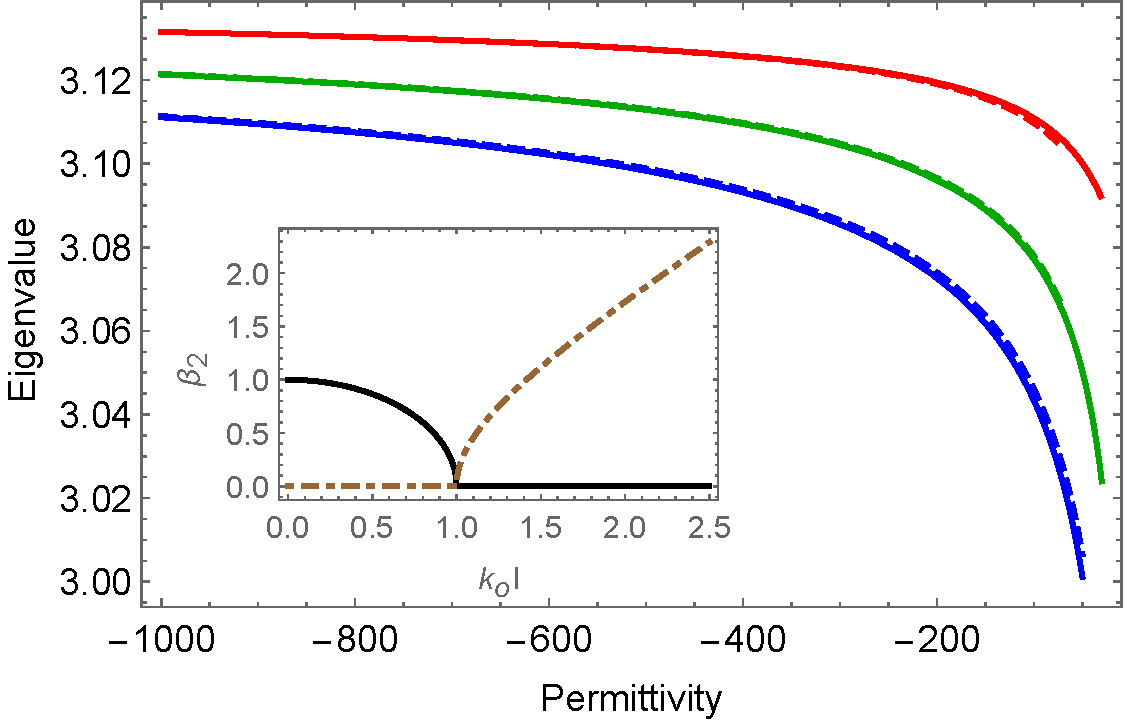
\includegraphics[width=0.8\columnwidth]{2nd_mode.pdf}
  \caption{Зависимость собственного значения $q_2\ell$ от значение диэлектрической проницаемости $\eps$ при $k_0 \ell = 1,2,3$ (снизу вверх):
  численный счёт (сплошная линия), асимптотическая формула (пунктирная линия). Во вставке приведена зависимость константы распространения 
  $\beta_2 \ell$ в зависимости от безразмерной ширины щели $k_0\ell$: вещественная часть (сплошная кривая), мнимая часть (штрихпунктир).}
  \label{fig:2nd_mode}
\end{figure}
Здесь чётные и нечётные $\nu$ соответствуют чётным и нечётным модам. Как и должно быть, главный член отвечает решению для идеального
проводника, в то время когда поправка порядка $O(\frac{1}{\sqrt{\abs{\varepsilon}}})$ для всех мод кроме фундаментальной $\nu = 0$, для 
неё $q_0 \sim \frac{1}{\abs{\varepsilon}^{1/4}}$. Приведём в пример частный случай сравнения вычисления одного собственного значения
вычисленного численным образом и приближённой формулой. На Рис.~\ref{fig:2nd_mode} представлена зависимость собственного значения $q_2\ell$ от 
диэлектрической проницаемости  $\eps$ для различных значений параметра $k_0 \ell = 1,2,3$, которая вычислена численно и используя 
приближённое выражение~(\ref{eq:Eigenvalues_approx}). Можно заметить, что разница между точным значением и приближённым возрастает с 
 $k_0 \ell$, а так же при увеличении $-\varepsilon$ значения сходятся к $\pi$, что и следовало ожидать. 

 Как только внимая часть проницаемости $\varepsilon'' \neq 0$, значение $q_\nu$ становится комплексной величиной, а соответствующая константа 
 распространения $\beta_\nu$ приобретает положительную мнимую часть и для распространяющихся мод в щели. Мнимая часть $\beta_\nu''$ определяет
 глубину проникновения моды $\nu$ в щель. Как только длина пластин вдоль оси $z$ становится много больше, чем характерная длина проникновения, то 
 есть $L_z \gg 1/\beta_\nu''$, мы можем пренебречь Френелевским отражением от границы $z = L_z$ и рассматривать только моду, распространяющуюся внутрь щели.  Как только $1/\min_{\nu}(\beta_\nu'') \ll L_z$,
 то длиной щели можно пренебречь в принципе для задачи. 

\subsection{Анализ вклада различных мод в щели в тензор Максвелла}

Давление электромагнитного поля описывается можно описать с помощью тензора натяжений Максвелла \begin{equation*}
    \sigma_{\alpha \beta} = \frac{1}{4 \pi}\Big( E_\alpha E_\beta + H_\alpha H_\beta - \frac{1}{2}\delta_{\alpha \beta}(E^2 + H^2) \Big)
\end{equation*}. Нас интересует давление электромагнитного поля по оси $x$ в точках $x = \pm l$, поэтому тензор натяжений приобретает следующий вид \textcolor{red}{Проверить коэффициент}
\begin{equation}
    \sigma_{xx} = \frac{1}{8 \pi} (\abs{E_x}^2 -\abs{E_z}^2 - \abs{H_y}^2).
\end{equation}

Рассмотрим ситуацию, когда в щели возбуждена лишь одна мода с индексом $\nu$, тогда
\begin{align*}
    H_y &= h_\nu b(q_\nu\ell) e^{i \beta_\nu z}  \\
    E_z &= \frac{i}{k_0} q_\nu h_\nu \frac{db}{dx}(q_\nu\ell) e^{i \beta_\nu z}  \\
    E_x &= \frac{1}{k_0} \beta_\nu h_\nu b(q_\nu\ell) e^{i \beta_\nu z}.
\end{align*}
Предполагая, что $\abs{\eps'} \gg 1$, мы можем пренебречь $E_z$, тогда давление будет иметь вид
\begin{equation}
   \sigma_{xx} \sim \abs{h_\nu}^2(\abs{\beta_\nu}^2 - k_0^2 )e^{-2\beta_\nu'' z}.
\end{equation}
Интегрируя данное выражение по всей поверхности щели, мы получаем вклад одной гармоники в плазмонную силу
\begin{equation}
  F \sim \abs{h_\nu}^2 (\abs{\beta_\nu}^2 - k_0^2)\frac{}{}
\end{equation}
\begin{equation*}
E_x = \frac{-i}{k_0}\frac{\partial H_y}{\partial z} = \frac{1}{k_0}\sum_{\nu}\beta_\nu h_\nu b_\nu(\ell) e^{i \beta_\nu z}
\end{equation*}
and 
\begin{equation*}
E_z = \frac{i}{k_0}\frac{\partial H_y}{\partial x} = \frac{i}{k_0}\sum_{\nu} q_\nu h_\nu  \frac{d b_\nu(\ell)}{d x} e^{i \beta_\nu z}.
\end{equation*}

\section{Сшивка полей при произвольном падении плоской волны}

 Граничные условия при $z = 0$ для тангенциальной составляющей полей $E_x^<(x,0) = E_x^>(x,0) $ и $H_y^<(x,0) = H_y^>(x,0)$ 
 позволяют найти неизвестные $a_k$ и $h_\nu$. Получающиеся уравнения
\begin{align}
\sum_{\nu = -\infty}^{+\infty} h_\nu b_\nu (x) = (1+R)e^{ik_{0x}x} 
+ \int a_{k'} e^{ik'x} dk', & \ \abs{x}<l, \label{eq:H} \\
\sum_{\nu = -\infty}^{+\infty} \beta_\nu h_\nu b_\nu(x) = (1-R)k_{0z}e^{ik_{0x}x}
- \int \varkappa a_{k'} e^{ik'x} dk', &\ \abs{x}<l,  \label{eq:Ex_in} \\
\sum_{\nu = -\infty}^{+\infty} c_\nu(x)\beta_\nu h_\nu b_\nu(l) e^{-q_{M\nu}\abs{x-l}} = 
 -\eps \int \varkappa a_{k'} e^{ik'x} dk', &\ \abs{x}>l. \label{eq:Ex_out}
\end{align}
Где коэффициент $c_\nu(x)$ равен единице для чётных мод и $\text{signum}(x)$ для нечётных, $q_{M\nu}^2 = \beta_\nu^2 - \eps k_0^2$
соответствует собственному значению моды $\nu$ в металле, и по сути является просто обратной длинной проникновения в стенки, так как 
является показателем в затухающей экспоненте. Уравнение~(\ref{eq:H}) обеспечивает непрерывность поля $H$ на входе в щель, 
уравнения.~(\ref{eq:Ex_in}) и~(\ref{eq:Ex_out}) обеспечивают непрерывность тангенциальной компоненты $E_x \sim \partial_{z} H_y$ при $z = 0$.

Умножая уравнения~(\ref{eq:Ex_in}) и~(\ref{eq:Ex_out}) на $e^{-ikx}$и интегрируя от $x = -\infty$ до $x = +\infty$  
мы выражаем $a_k$ через $h_\nu$:
\begin{align}
a_k = \frac{k_{0z}l }{\pi \varkappa} (1-R)\sinc((k_{0x}-k)l) 
        - \frac{l}{2 \pi \varkappa}\sum_{\nu = -\infty}^{+\infty} \beta_\nu h_\nu\left[f_{q_\nu,k}
+ \frac{b_\nu(l)}{\eps}G(q_\nu,k)\right],
\end{align}
где $f_{q_\nu,k}$ и $G(q_\nu,k)$ определены как 
\begin{align*}
&f_{q_\nu,k} =
\sinc(q_\nu-k)l + \sinc(q_\nu+k)l,\\
&G(q,k) = 2\frac{q\cos{kl}+k\sin{kl}}{q^2 + k^2}\\
\end{align*}
для чётных мод,
\begin{align}
&f_{q_\nu,k} = i\ \sinc(q_\nu-k)l - i\ \sinc(q_\nu+k)l,\nonumber\\
& G(q,k) = -2\frac{q\sin{kl}+k\cos{kl}}{q^2 + k^2}
\end{align}
для нечётных.
Здесь использовано обозначение  $\sinc(x) = {\sin{x}}/{x}$.

Теперь мы подставляем $a_k$ в уравнение~(\ref{eq:H}) чтобы найти $h_\nu$. Умножая полученное уравнение на  $\cos{q_\mu x}$ ($\sin{q_\mu x}$) 
и интегрируя от $x = -l$ до $x = l$ мы получаем систему линейных уравнений на $h_\nu$. Благодаря разным чётностям мод полная система
разбивается на две независимые для чётных и нечётных по отдельности. Система уравнений на коэффициенты при чётных модах 
\begin{align}
	\sum_{\nu=-\infty}^{+\infty} F_{\mu \nu} h_\nu = (1+R)f_{\mu,-k_{0x}} + \frac{(1-R)k_{0z} l}{\pi}\int f_{\mu,-k}\sinc((k_{0x}-k)l) \frac{dk}{\varkappa}; \label{eq:General_System}
\end{align}
где 
\begin{align}
F_{\mu \nu} &= f_{\mu,\nu} + \frac{\beta_\nu}{2\pi}\int
\Bigl(f_{\nu,k}f_{\mu,-k}  + \frac{b(l)}{\eps} G(q_{M\nu},k)f_{\mu,-k} \Bigr)\frac{dk}{\varkappa}.
\label{eq:F_mn}
\end{align}
Для нечётных мод нужно лишь умножить первый член $f_{\mu,\nu}$ in~(\ref{eq:F_mn}) на $-i$ и взять соответствующие функции. 

При стремлении $\eps \to -\infty$, второй член под знаком интеграла стремится к нулю как $\abs{\varepsilon}^{-3/2}$, 
учитывая, что собственные значения симметричны $q_{\nu} = -q_{-\nu}$, то можно проводить суммирование в уравнении~(\ref{eq:General_System}) 
от $\nu = 0$ до $+\infty$, учитывая каждую моду $\nu \neq 0$ с коэффициентом $2$. В итоге, предельный переход даёт ту же систему
уравнений что в работе~\cite{Shapiro16}.

Эта система уже позволяет анализировать по отдельности эффекты непараллельного падения излучения на щель и влияния высших гармоник на силу
при для широкой щели, когда условие $k_0 \ell \ll 1$ не выполняется.

\subsection{Предельный переход к идеальному проводнику}

\subsection{Наклонное падение}

\subsection{Вклад высших мод при нормальном падении}
Для начала мы сравним результаты для реального и идеального металлов. Выбрав значение проницаемости $\eps = -100 + 10i$, которая соответствует 
проницаемости золота при $k_0 = 1.5$ мкм, мы вычисляем значение амплитуды магнитного поля на входе в зазор $\abs{H(0,0)}^2$ в зависимости от 
безразмерной ширины $k_0 \ell$ в случае нормального падения излучения. Так как в работе~\cite{Shapiro16} было показано, что при 
$k_0 \ell \sim 1$ достаточно учитывать лишь две высшие моды, мы вычисляем лишь значения $h_0$ и $h_2$.

\begin{figure}
  \begin{subfigure}[t]{0.45\textwidth}
    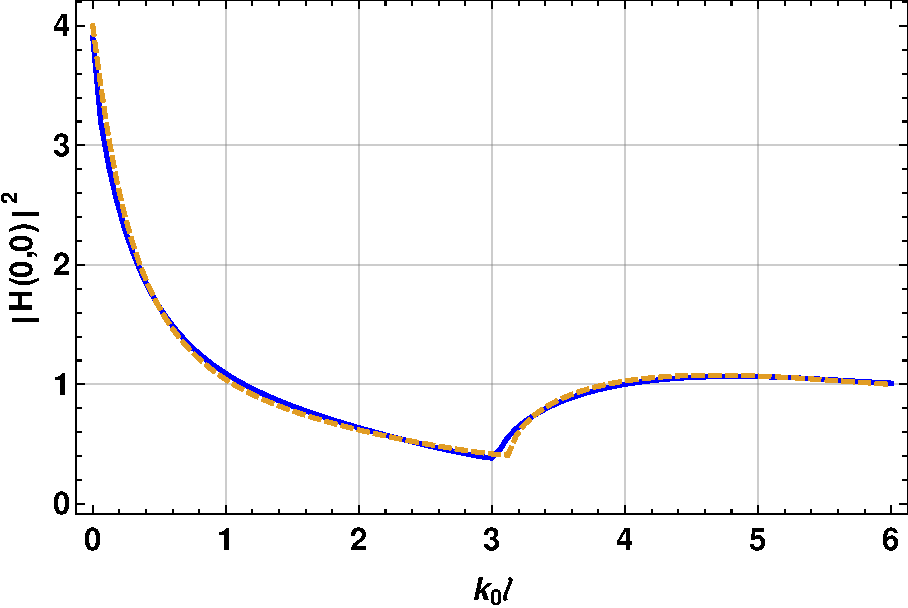
\includegraphics[width=1\textwidth]{H00_2modes_com.pdf}
  \end{subfigure}
  \begin{subfigure}[t]{0.45\textwidth}
    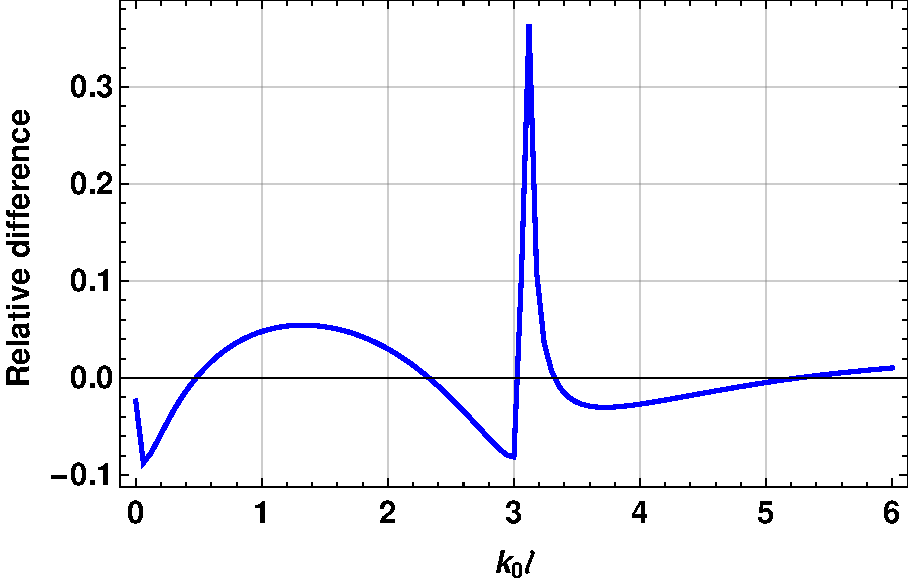
\includegraphics[width=1\columnwidth]{H00_2modes_comp_rel.pdf}
  \end{subfigure}
  \caption{(a) Зависимость $\abs{H(0,0)}^2$ от $k_0 \ell$. Сплошная линия соответствует конечному $\eps$, пунктир идеальному проводнику. (b) Относительная разница.}	\label{pic:comp}
\end{figure}

На Рис.~\ref{pic:comp} показана зависимость $\abs{H(0,0)}^2$ от $k_0 \ell$ в сравнении с идеальным проводником. Можно заметить, что в целом 
относительная разница не превышает  $10\%$ и лишь при  $k_0 \ell \approx \pi$ достигает $40\%$. Физически эта точка 
соответствует порогу рождения второй моды, а порог рождения, как было показано выше, <<смещается>> при учёте конечной проводимости, и фактически
вблизи этой точки возникает ситуация, когда вторая мода для реального металла уже становится распространяющейся (Рис.~\ref{fig:2nd_mode}), 
в то время как для идеально проводника
она ещё остаётся эванесцентной, отсюда и происходит такая большая относительная разница. Однако стоит заметить, что в целом картина сохраняется
и учёт конечной проводимости в расчёте амплитуд $h_\nu$ даёт ответ отличающийся не больше чем на $10\%$, но с другой стороны этот учёт 
становится дорогостоящим с точки зрения численного интегрирования интегралов, которые стоят как коэффициенты в системе линейных уравнений.

Силу, действующую на стенки в присутствии электромагнитного излучения, определяет тензор Максвелла. В данной задаче, его усредненное по
периоду выражение даётся формулой
\begin{equation}
\bar{\sigma}_{xx} = \abs{E_x}^2 - \abs{E_z}^2 - \abs{H_y}^2,
\end{equation}
где поля 
\begin{equation*}
E_x = \frac{-i}{k_0}\frac{\partial H_y}{\partial z} = \frac{1}{k_0}\sum_{\nu}\beta_\nu h_\nu b_\nu(x) e^{i \beta_\nu z}
\end{equation*}
и
\begin{equation*}
E_z = \frac{i}{k_0}\frac{\partial H_y}{\partial x} = \frac{i}{k_0}\sum_{\nu} q_\nu h_\nu  \frac{d b_\nu(x)}{d x} e^{i \beta_\nu z}.
\end{equation*}

\section{Учёт конечных размеров пучка по оси $x$}
\subsection{Влияние ширины пучка на высшие моды}

\chapter{Решение в трёхмерном случае для Гауссова пучка}
\section{Приближение узкой щели}

\chapter{Сравнение с экспериментальными результатами}
